% vim: set tw=78 tabstop=4 shiftwidth=4 aw ai:

\chapter{Peer-to-Peer Systems and Protocols}
\label{chapter:p2p-systems}

Termenul Peer-to-Peer (P2P) a devenit un "buzzword" la începutul secolului 21
și reprezintă actualmente una dintre cele mai întâlnite tehnologii. Dacă până
în anul 2000 paradigma cea mai folosită în Internet era client-server, o dată
cu apariția Napster, tehnologia Peer-to-Peer a devenit una dintre cele mai
folosite și mai controversate tehnologii.

Cu un număr de 60 de milioane de utilizatori în 2001 și partajarea  a multor
terraocteți de muzică Napster a devenit rapid centrul atenției publice și
promotorul tehnologiei P2P. Curând după, o serie întreagă de soluții
Peer-to-Peer au dus la o nou mod de a partaja informații, fișiere, cunoștințe,
date (JXTA, Gnutella, BitTorrent, DirectConnect, Jabber).

În traducere liberă, "peer-to-peer" înseamnă comunicare între egali, adică
între două entități autonome și independente una de cealaltă. Principial, un
sistem "Peer-to-Peer" este un sistem descentralizat: fiecare nod din rețea are
același rol ca oricare alt nod. Opusul este sistemul client server care este
centralizat pe server. Un avantaj imediat al arhitecturilor Peer-to-Peer este
scalabilitatea și toleranța la defecte.

În principiu, un sistem este considerat "peer-to-peer" dacă răspunde afirmativ
la următoarele întrebări:
\begin{itemize}
  \item Tratează conectivitatea variabilă și adresele temporare ca pe un lucru
  firesc?
  \item Oferă nodurilor de la marginea rețelei autonomie vizibilă?
\end{itemize}

În plus, există o a treia condiție, implicită, care precizează că trebuie să
existe comunicație între noduri pentru ca sistemul să funcționeze.

Se observă că aceste condiții nu impun o arhitectură descentralizată, așa cum
este perceput de obicei un sistem peer-to-peer. Condițiile presupun că fiecare
nod al rețelei este mai mult sau mai puțin un jucător independent și nu este
necesar pentru ca întreg sistemul să funcționeze.  Istoria sistemelor
Peer-to-Peer și a Internet-ului

Internet-ul este o resursă partajată, un rezervor de informație și o rețea
cooperativă construită din milioane de noduri în întreaga lume. Începând cu
anii '90, Internet-ul a cunoscut o creștere explozivă, lucru care a dus la o
cerere acută pentru una din resursele fundamentale: lățimea de bandă.
Necesitatea ca Internetul să suporte o gamă largă de aplicații deținând
constrângeri de securitate a dus la apariția de firewall-uri care au împărțit
Internet-ul în mai multe părți.

Totuși, în anul 2000, totul s-a schimbat, sau, mai bine, spus, a revenit la
condiția inițială. Ceea ce până atunci erau elemente pasive au devenit
elemente active. Prin intermediul aplicației de partajare de fișiere de muzică
(Napster) și a unei mișcări mai largi (denumită peer-to-peer), milioanele de
utilizatori conectați la Internet au început să-și folosească sistemele de
calcul din ce în ce mai puternice de acasă pentru mai mult decât browsing și
citrea e-mail-urilor. Sistemele conectate prin intermediul Internet-ului
puteau forma grupuri și colabora pentru satisfacerea diverselor nevoi.

\section{Evolution of the Internet}
\label{sec:p2p-systems:evolution-internet}

\subsection{Eary Internet (1969-1995)}

Internet-ul proiectat inițial în cadrul proiectului ARPA era un sistem
peer-to-peer. Primele câteva noduri din ARPANET nu erau conectate într-o
relație client-server, ci într-o relație de egalitate. Totodată, Internet-ul
din acea perioadă era mult mai deschis și liber decât Internet-ul din ziua de
azi. Firewall-urile erau necunoscute și oricare două sisteme din Internet își
puteau transmite pachete unul altuia.

Primele aplicații importante din Internet erau poșta electronică (e-mail), FTP
și telnet. Deși aplicațiile urmau paradigma client/server, cazurile de
utilizare erau simetrice. Fiecare stație din Internet putea folosi telnet sau
FTP pentru a se conecta la oricare altă stație.

Această simetrie a Internet-ului a permis existența unor sisteme complexe
precum Usenet sau DNS care folosesc mecanisme de comunicare peer-to-peer. În
anii ce au urmat, Internet-ul a devenit din ce mai restrâns la aplicații de
tip client/server. Totuși, o dată cu apariția aplicațiilor de tip
peer-to-peer, tendința este ca Internet-ul să revină la proiectarea inițială.

\subsection{Internet Expansion (1995-1999)}

Explozia Internet-ului din anul 1994 a schimbat radical fața acestuia.
Milioane de oameni au început să folosească Internet-ul. Unde până atunci
Internet-ul era un obiect de studiu pentru oamenii de știință preocupați de
rețele complexe de calculatoare, acum oameni obișnuiți au devenit interesați
de Internet pentru a trimite mesaje, a vedea pagini web sau a cumpăra diverse
articole.

Schimbarea Internet-ului într-un fenomen cultural de masă a avut un impact
foarte mare asupra arhitecturii retelelor. Schimbările se reflecta în
împărțirea colaborării pe Internet, folosirea pe scară din ce în ce mai largă
a firewall-urilor.

Creșterea spectaculoasă a Internet-ului, apariția de aplicații ale căror
principale ținte erau sistemele cu legătură slabă la Internet, folosirea de
firewall-uri și NAT au condus la proliferarea modului client/server al
Internet-ului. Browser-ul web era o aplicație simplă care se baza pe un
protocol client/server la fel de simplu: clientul cere o pagină, server-ul i-o
oferă, după care conexiunea se închide. Sistemul pe care se găsește clientul
nu trebuie să aibă o adresă permanentă sau o adresă binecunoscută.

Perioada exploziei Internet-ului a fost caracterizată de spargerea modului de
colaborare pentru care fusese inițial proiectat Internet-ul. Firewall-urile,
adresele IP dinamice, folosire NAT sunt tehnologiile care au dus la o
împărțire strictă a stațiilor din Internet în servere și clienți. Rezultatul
direct este că multe stații din Internet sunt greu accesibile. Aplicații
peer-to-peer precum sistemele de mesagerie sau de file-sharing trebuie să
lucreze intens pentru a trece de aceste limitări.

\subsection{Rebirth of the Peer-to-Peer Paradigm}

Începând cu anul 2000 (Napster), aplicațiile peer-to-peer au devenit din ce în
ce mai comune și mai utilizate. Aplicațiile peer-to-peer permit publicarea
facilă a informațiilor și permit proiectarea de aplicații descentralizate,
lucru care este simultan o provocare și o oportunitate.

În speță, modelul peer-to-peer este strâns corelat cu ideea de
descentralizare. Într-un sistem total descentralizat, fiecare nod este un
participant egal fără a exista stații cu roluri speciale. DNS este un protocol
proiectat ca model peer-to-peer care are însă implicită ideea de ierarhie.
Multe alte sisteme peer-to-peer dețin o organizare semicentralizată în care
anumite noduri au roluri speciale.

Totuși, aplicațiile peer-to-peer se lovesc de mai multe probleme în
arhitectura curentă a Internet-ului: firewall-urile, NAT îngreunează procesul
de conectare între stații. Lățimea de bandă asimetrică împiedică utilizatorii
să servească fișierele de pe sistemele proprii cât mai eficient.

Dincolo de problemele tehnice, aplicațiile peer-to-peer se lovesc de probleme
de natură socială. Partajarea fișierelor într-un sistem peer-to-peer trebuie
să țină cont de free-riders. Cei care folosesc fișiere partajate de alții fără
a partaja nimic. Pentru aceasta trebuie să existe o formă de contabilizarea a
efortului depus de fiecare client.

De asemenea, încă de la lansarea Napster, aplicațiile peer-to-peer au atras
multe probleme legale legate de copyright-ul materialelor și de partajarea
lor. Aici ne referim la fișiere audio, video, documentație electronică et.

\section{The Peer-to-Peer Paradigm}
\label{sec:p2p-systems:paragigm}

\subsection{Features and Models of Peer-to-Peer Systems}

După cum s-a amintit și anterior, caracteristicile rețelelor P2P sunt
partajarea și distribuirea resurselor, descentralizarea și autonomia.

Partajarea și distribuirea resurselor se referă la modul în care funcționează
fiecare nod al rețelei peer-to-peer. Un nod are funcționalitate atât de server
cât și de client și poate acționa atât ca furnizor cât și ca un conumator de
resurse și servicii (informație, fișiere, lățime de bandă, spațiu de stocare,
cicluri de procesor). Aceste noduri se mai numesc și servanți.

Descentralizarea se referă la absența unei autorități centrale coordonatoare
pentru organizarea rețelei sau pentru folosirea resurselor și a comunicațiilor
între nodurile rețelei. Comunicația are loc direct între noduri. În mod
frecvent, există o distincție între rețele P2P pure și rețele hibride. În
rețelele P2P hibride, anumite funcții (precum indexarea și autentificarea)
sunt alocate unui subset de noduri care folosesc rolul de entitate
coordonativă.

Autonomia înseamnă că fiecare nod al rețelei decide independent ce resurse să
furnizeze celorlalte noduri.

Scăderea costurilor pentru ciclurile de procesor, lățime de bandă, spațiu de
stocare, cumulate cu creșterea Internet-ului au creat noi arii de aplicare a
rețelelor P2P. Acest lucru a condus la o creștere explozivă a aplicațiilor P2P
și discuții legate de limitări, performanță și implicațiile economice, sociale
și legale. Figure~\ref{fig:p2p-systems:p2p-levels} este prezentat un model pe
trei niveluri cuprins din infrastructuri P2P, aplicații și comunități cu
scopul de a rezolva lipsa de claritate legată de terminologia P2P.

\begin{figure}
  \centering
  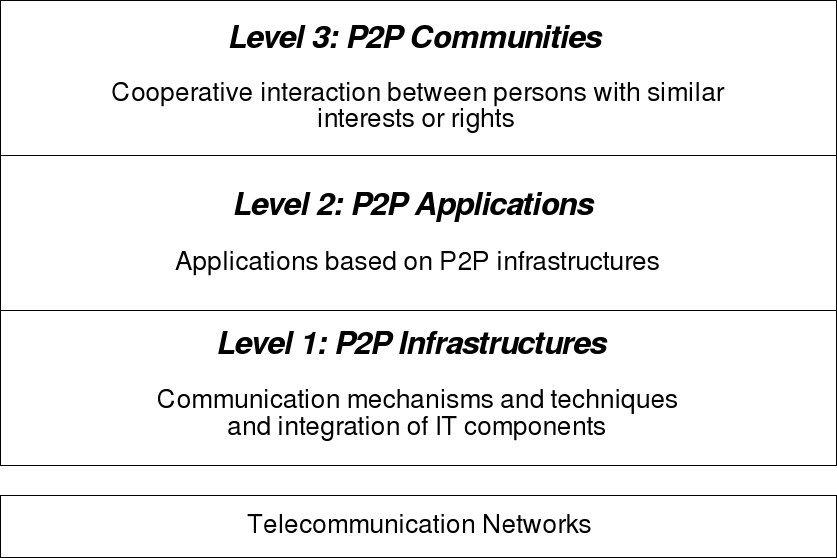
\includegraphics[width=0.7\textwidth]{src/img/p2p-systems/p2p-levels}
  \caption{Peer-to-Peer Levels}
  \label{fig:p2p-systems:p2p-levels}
\end{figure}

Infrastructurile P2P sunt poziționate deasupra rețelelor de comunicație
existente și acționează ca un fundament pentru celelalte niveluri.
Infrastructurile P2P furnizează comunicație, integrare și translatare între
diversele componente IT. Furnizează, de asemenea, servicii de căutare și de
comunicație între nodurile rețelei, de identificare și partajare a resurselor,
ca și inițierea de procese de securitate precum autentificarea și autorizarea.

Nivelul 2 este reprezentat de aplicațiile P2P care folosesc serviciile
infrastructurilor P2P. Aplicațiile sunt folosite pentru a permite comunicația
și colaborarea între diferitele entități în absența unui control central.

Nivelul 3 se concentrează pe fenomenul de interacțiune socială; în particular,
pe construirea de comunități și dinamica acestora.

\subsection{P2P Resource Management}

În literatura de specialitate, aplicațiile P2P sunt adesea clasificate în
categorii precum: instant messaging, partajarea fișierelor, grid computing și
colaborare. Acest mod de clasificare s-a dezvoltat de-a lungul timpului și nu
reușește să facă distincții clare între diversele aplicații. În ziua de azi,
există situații multe dintre categorii pot fi considerate echivalente. Din
aceste motive, o altă clasificare poate lua în considerare aspectele legate de
resursele folosite în sistemele P2P.

Există, așadar o clasificare a sistemelor P2P conform cu resursele
disponibile.

\subsubsection{Data}

Informația este folosită în spațiile colaborative în forma partajării sau
schimbului de informație și a management-ului documentelor. Informația legată
de prezența nodurilor în sistemele P2P este fundamentală pentru organizarea
sistemului P2P și pentru a cunoaște date despre noduri și despre resursele pe
care aceștia le pun la dispoziție. Informația de prezență este utilă pentru a
cunoște ciclurile de procesor libere pe un sistem de calcul care pot fi
folosite într-o aplicație de tip grid.

DMS (Document Management Systems) sunt spații de stocare organizate central
care permit stocarea partajată, managementul și utilizarea datelor. Rezultat
al aplicațiilor de partajare a informațiilor (P2P groupware) este formarea de
grupuri colaborative pentru management-ul documentelor. In sistemele groupware
server/client, trebuie creat un spațiu de lucru pentru management-ul
informației. Un sistem P2P poate evita toate sarcinile legate de administrarea
acelui spațiu de lucru.

\subsubsection{Files}

Partajarea fișierelor reprezintă forma cea mai întâlnită de aplicații P2P. Se
apreciază că circa 70\% din traficul Internet-ului poate fi atribuit schimbului
de fișiere (mai ales fișiere media). Una din problemele principale ale
sistemelor P2P (și a aplicațiilor de partajare a fișierelor) este localizarea
resurselor. În contextul sistemelor de partajare a fișierelor s-au dezoltat
trei algoritmi: modelul de flood, modelul de director centralizat și modelul
dirijării documentelor. Aceste modele sunt ilustrate cel mai bine de
implementările proeminente: Gnutella, Napster și Freenet.

\subsubsection{Bandwidth}

O dată cu creșterea cererii pentru capacitățile de transmitere a rețelelor
datorată în principal creșterii volumului de transfer multimedia, folosirea
efectivă a lățimii de bandă devine din ce în ce mai importantă. De obicei,
abordările centralizate în care fișierele sunt ținute pe server duc la
apariția de bottleneck-uri în sistem în momentul sosirii simultane de
solicitări de la mai mulți clienți.

În aceste situații, folosirea sistemelor P2P are două avantaje: creșterea
echilibrării încărcării (load balancing) prin folosirea rutelor de transmisie
care nu erau exploatate; folosirea partajată a lățimii de bandă care permit
accelerarea descărcării și transportului fișierelor mari solicitate simultan
de diverse entități. În general aceste fișiere sunt împărțite în blocuri mai
mici descărcate simultan de la diverse noduri ale rețelei.

\subsubsection{Storage}

Creșterea conectivității și disponibilitatea crescândă a lățimii de bandă
permit forme alternative de management a spațiului de stocare care rezolvă
aceste probleme și necesită mai puțin efort administrativ. În rețelele de
stocare P2P, doar o porțiune din spațiul unui desktop PC va fi utilizat. O
rețea de stocare P2P este un cluster de calculatoare format pe baza unor
rețele existente care partajează spațiul de stocare existent în rețea. Când un
fișier este stocat în rețea i se asociază un număr de identificare unic
obținut prin aplicarea unei funcții hash asupra numelui sau conținutului
fișierului. În plus, se stochează și un număr dat de copii ale fișierului.

\subsubsection{CPU Cycles}

Recunoașterea faptului că există putere de calcul nefolosită într-o rețea de
calculatoare a condus la încrederea în aplicații P2P care să folosească acea
putere. Folosirea aplicațiilor P2P pentru colectarea ciclurilor de procesor,
se poate atinge o putere de calcul care poate fi furnizată foarte greu chiar
și de cele mai scumpe supercalculatoare. Această formă de abordare a folosirii
coordonate de resurse de calcul distribuite în organizații virtuale, dinamice
care se extind dincolo de o simplă instituție intră sub auspiciile domeniului
"grid computing".

Unul dintre cele mai folosite exemple de proiect grid în contexul rețelelor
P2P este SETI@home. SETI@home este o inițiativă științifică lansată de
Universitatea din California, Berkeley, cu scopul de descoperire a semnalelor
radio ale inteligenței extraterestre. Pentru acest scop, un telescop radio din
Puerto Rico înregistrează o porțiune din spectrul electromagnetic din spațiu.
Datele sunt transmise serverului central din California. În loc de a analiza
datele folosind un supercalculator, serverul împarte informația în unități
mici și le trimite pentru procesare milioanelor de calculatoare care s-au
oferit voluntare pentru participarea la acest proiect.

\subsection{P2P Topologies for File Sharing}

Topologia unei rețele P2P se referă la modul de conectare a nodurilor,
existența unui nod/noduri specializate și modul de transfer a fișierelor
partajate sau a metainformațiilor. Din punct de vedere al topologiei rețelei,
sistemele P2P au două caracteristici principale:

\begin{itemize}
  \item scalabilitatea: nu există o limitare tehnică sau algoritmică a
  dimensiunii sistemului; complexitatea sistemului trebuie să fie relativ
  constantă raportat la numărul de noduri din sistem
  \item fiabilitatea (reliability): lipsa de funcționare a unui nod dat nu va
  afecta întregul sistem (sau, posibil, nici alte noduri)
\end{itemize}

Sistemele P2P pot fi grupate în două categorii: sisteme P2P pure și sisteme
P2P hibride. Sistemul P2P pur (precum Gnutella sau Freenet) nu are un server
central. Modelul hibrid P2P, precum Napster, eDonkey2000, Groove, folosește un
server central pentru a obține metainformație precum identitatea nodului unde
se găsește o anumită resursă sau pentru verificarea de informații credențiale.
Într-un sistem hibrid, nodurile contactează mereu un server central înainte de
a contacta direct alte noduri.

Toate topologiile P2P, indiferent de deosebiri, au o caracteristică comună:
toate transferurile de informație între noduri se realizează prin conexiuni
directe între noduri. Totuși, controlul procesului înainte de transferul
fișierului poate fi implementat în mai multe moduri. Drept urmare, rețelele
P2P pot fi clasificate în 4 categorii importante: centrlizate,
descentralizate, ierarhice și inel. Deși aceste topologii pot exista de sine
stătătoare, în practică sistemele distribuite dețin topologii mai complexe
prin combinarea câtorva sisteme de bază pentru crearea a ceea ce se cheamă
sistem hibrid.

\subsubsection{Centralized}

Conceptul topologiei centralizate se bazează pe modelul tradițional
client/server. Trebuie să existe un server centralizat care este folosit
pentru a controla fișierele și bazele de date cu utilizatorii nodurilor care
intră în sistem. Clientul contactează serverul pentru a-l informa de adresa IP
curentă și numele fișierelor pe care dorește să le partajeze. Acest lucru se
realizează ori de câte ori aplicația este lansată. Informația colectată de la
noduri va fi apoi folosită de server pentru a crea o bază de date centralizată
dinamică care mapează numele de fișiere unor seturi de adrese IP.

\begin{figure}
  \centering
  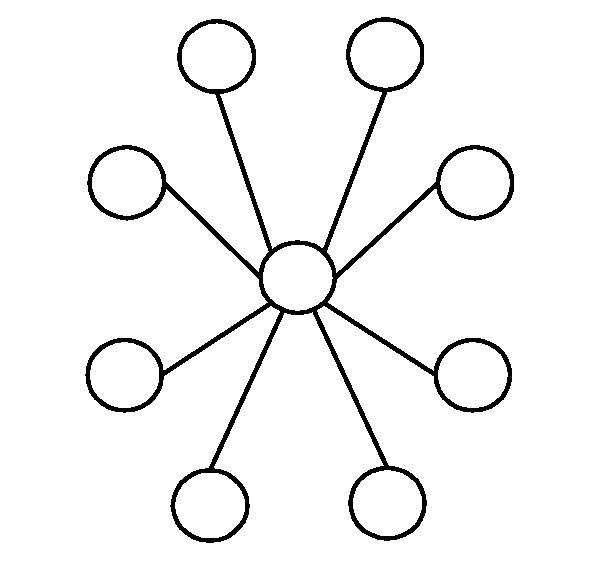
\includegraphics[width=0.4\textwidth]{src/img/p2p-systems/centralized}
  \caption{Centralized Topology}
  \label{fig:p2p-systems:centralized}
\end{figure}

Toate cererile de căutare sunt adresate serverului care va consulta baza de
date locală. Dacă are loc o potrivire se creează o legătură directă către
nodul care partajează fișierul și se execută transferul. În nici o situație
fișierul partajat nu va fi prezent pe server.

\subsubsection{Ring}

Dezavantajul important al topologiei centralizate este faptul că serverul
central poate deveni un bottleneck în sistem (în cazul unei încărcări
semnificative) și un punct critic în cazul unei defecțiuni. În aceste
contexte, a apărut topologia de tip inel.

\begin{figure}
  \centering
  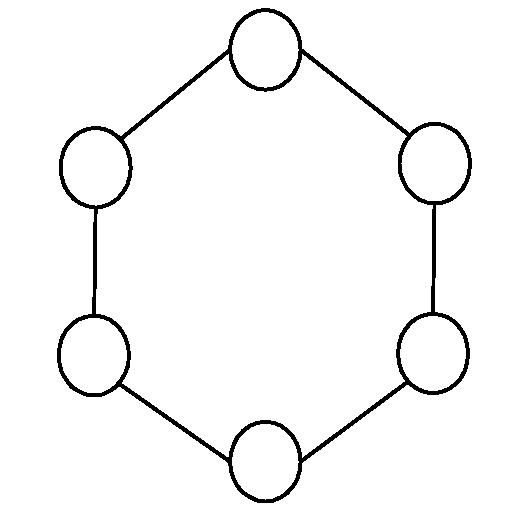
\includegraphics[width=0.4\textwidth]{src/img/p2p-systems/ring}
  \caption{Ring Topology}
  \label{fig:p2p-systems:ring}
\end{figure}

Topologia de tip inel este realizată dintr-un cluster de sisteme care sunt
aranjate în forma unui inel care să acționeze ca un server distribuit. Acest
cluster conlucrează pentru a furniza o echilibrare a încărcării cât mai bună
și pentru disponibilitate cât mai ridicată. Această topologie este în mod
obișnuit folosită când toate sistemele sunt relativ apropiate topologic și
sunt, destul de probabil, deținute de o singură organizație unde anonimitatea
nu este de o importanță deosebită.

\subsubsection{Hierarchical}

Topologia ierarhică există încă de la începului civilizației umane. Cel mai
cunoscut exemplu de sistem ierarhic din Internet este DNS (Domain Name
System). Autoritatea se translatează de la server-ele de nume rădăcină până la
server-ele numelui înregistrat. Topologia este potrivită sistemelor care
necesită o formă de guvernare ce implică delegarea de drepturi sau de
autoritate. Un alt exemplu este cel al autorităților de certificare (CA) care
certifică validitatea unei intrări în Internet.

\begin{figure}
  \centering
  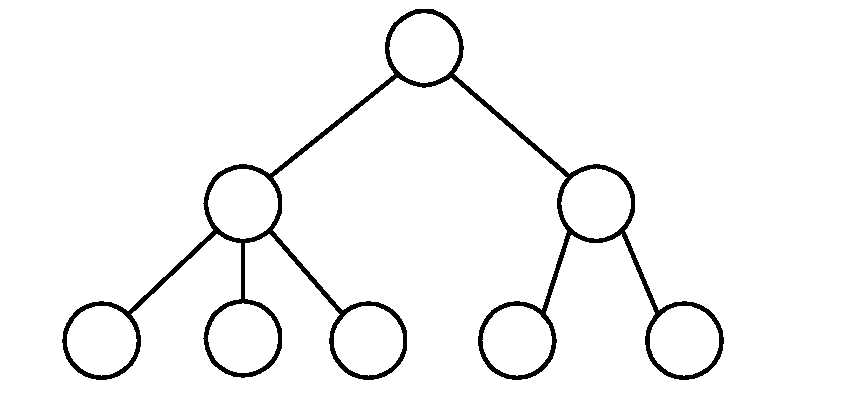
\includegraphics[width=0.4\textwidth]{src/img/p2p-systems/hierarchical}
  \caption{Hierarchical Topology}
  \label{fig:p2p-systems:hierarchical}
\end{figure}

\subsubsection{Fully Decentralized}

Într-o arhitectură P2P pură, nu există servere centralizate. Toate nodurile
sunt egale rezultând în obținerea unei topologii plate, nestructurate. Pentru
a se alătura rețelei un nod trebuie să contacteze un nod de bootstrap (nod
care este permanent online). Acesta îi va oferi nodului nou intrat adresele IP
ale unuia sau mai multor noduri, făcându-l oficial parte a rețelei dinamice.
Fiecare nod, totuși, va deține numai informație despre vecinii săi – nodurile
cu care are legătură directă în cadrul rețelei.

\begin{figure}
  \centering
  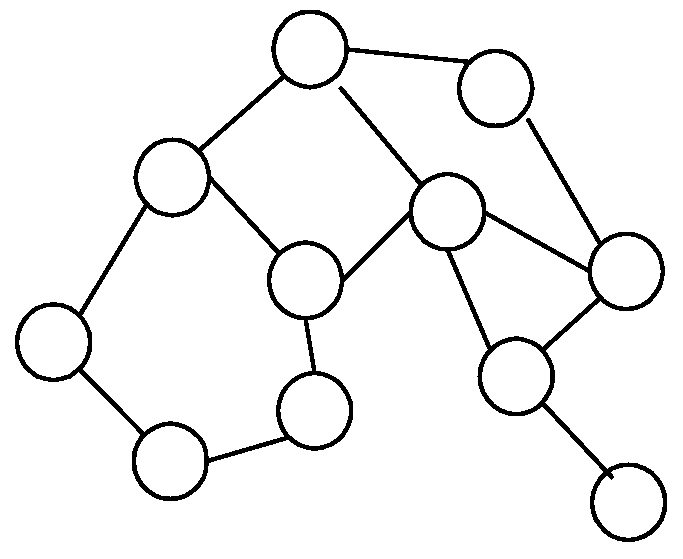
\includegraphics[width=0.4\textwidth]{src/img/p2p-systems/decentralized}
  \caption{Fully Decentralized Topology}
  \label{fig:p2p-systems:decentralized}
\end{figure}

Întrucât nu există servere care să controleze căutările, cererile pentru
fișiere sunt trimise în formă de flood prin intermediul rețelei. Flooding-ul
are drept consecință o încărcare suplimentară a lățimii de bandă a rețelei.

\subsubsection{Hybrid}

În ziua de astăzi, rețelele P2P combină multe dintre topologiile de bază de
mai sus. Acestea se mai numesc și arhitecturi hibride. În astfel de sisteme,
nodurile vor juca de obicei mai multe roluri.

\subsubsection{Centralized Ring}

Această topologie hibridă este foarte comună în cazul sistemelor de Web
hosting. După cum s-a menționat anterior, serverele Web dețin de obicei un
inel de servere specializate în echilibrarea încărcării și toleranța la
defecte. Astfel, serverele sunt dispuse într-o topologie de tip inel. Clienți
sunt conectați inelului de servere prin intermediul unei topologii
centralizate.

\begin{figure}
  \centering
  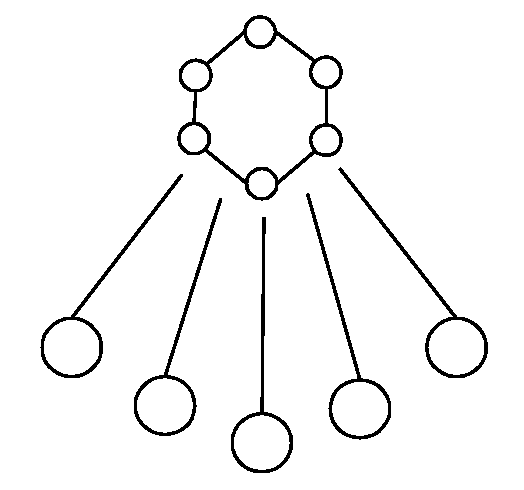
\includegraphics[width=0.4\textwidth]{src/img/p2p-systems/centralized-ring}
  \caption{Centralized Ring Topology}
  \label{fig:p2p-systems:centralized-ring}
\end{figure}

\subsubsection{Centralized-Centralized}

Se poate întâmpla adesea ca un server al unei rețele să fie el însuși un
client al unei rețele mai mari. Acest tip de topologie hibridă este foarte
comună în organizații care furnizează servicii Web.

\begin{figure}
  \centering
  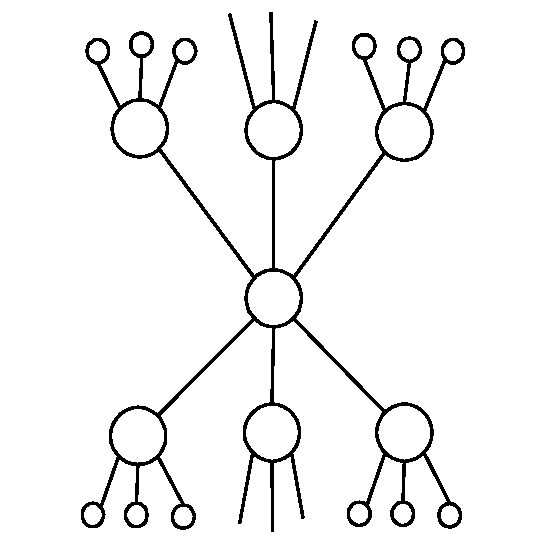
\includegraphics[width=0.4\textwidth]{src/img/p2p-systems/centralized-centralized}
  \caption{Centralized-Centralized Topology}
  \label{fig:p2p-systems:centralized-centralized}
\end{figure}

\subsubsection{Centralized-Decentralized}

În această topologie există noduri care funcționează ca lideri de grup. De
obicei se cheamă SuperNoduri. SuperNodurile furnizează sarcinile unui server
centralizat dar numai într-un subset de noduri. SuperNodurile sunt conectate
într-un mod descentralizat.

\begin{figure}
  \centering
  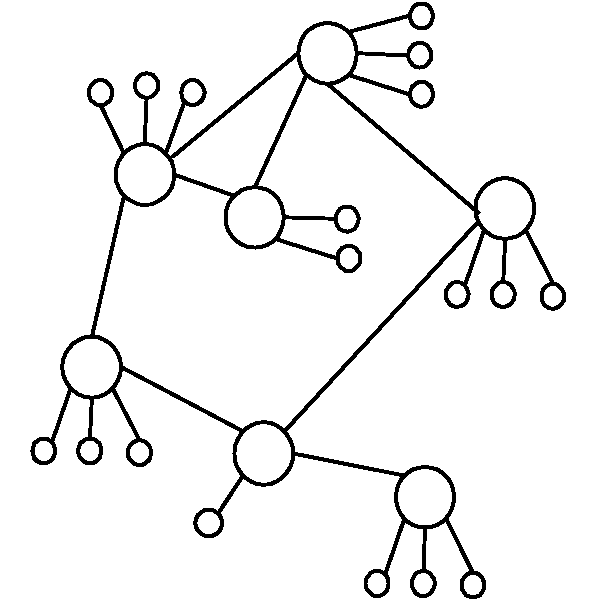
\includegraphics[width=0.4\textwidth]{src/img/p2p-systems/centralized-decentralized}
  \caption{Centralized-Decentralized Topology}
  \label{fig:p2p-systems:centralized-decentralized}
\end{figure}

La fel ca într-o topologie centralizată, SuperNodurile mențin o bază de date
care mapează fișierele la adrese IP a tuturor nodurile care sunt asociate.
Baza de date a SuperNodurilor menține informații doar despre grupul de noduri.
Un model de aplicație P2P care folosește o astfel de topologie este FastTrack.
Un alt exemplu de astfel de topologie este sistemul de e-mail de Internet.

\section{Peer-to-Peer Systems in the Internet}
\label{sec:p2p-systems:p2p-internet}

\subsection{Napster}

Napster a fost primul exemplu de succes de sistem peer-to-peer. Rularea
Napster s-a închis definitiv în iunie 2001 marcând încheierea unei epoci
remarcabile în care serviciul înregistrase 65 de milioane de utilizatori în
numai de 20 de luni. Napster are un model de control central care este posibil
datorită abordării centrate pe utilizator.

Figure~\ref{fig:p2p-systems:napster} prezintă prezintă componentele esențiale
ale arhicturii Napster în care comunicația este mediată de server. Clienții se
conectează intern la un "metaserver" cunoscut intern care acționează ca un
arbitru de conexiune. Metaserver-ul asociază un server cu încărcare redusă
dintr-unul din clustere. Serverele sunt în număr de 5 într-un cluster și pot
controla accesul a circa 15.000 de utilizatori.

\begin{figure}
  \centering
  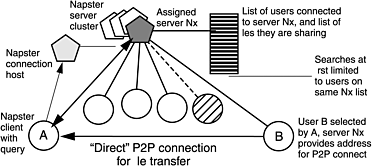
\includegraphics[width=0.7\textwidth]{src/img/p2p-systems/napster}
  \caption{Napster Architecture}
  \label{fig:p2p-systems:napster}
\end{figure}

Clientul se înregistrează în continuare serverului asociat furnizându-i
identitatea și informații despre fișierele partajate pentru baza de date.
Clientul recepționează informații legate de alți utilizatori conectați și
fișiere disponibile. Utilizatorii sunt practic anonimi unul față de celălalt,
directorul utilizatorului nefiind interogat direct. Interesul principal este
căutarea conținutului și determinarea nodului de unde să fie descărcată
resursa. Directorul de pe server folosește doar ca un serviciu de translatare
între identitatea stației asociată cu resursa dorită și adresa IP necesară
pentru inițierea unei conexiuni către client.

Performanța rețelei este esențială și de aceea căutările sunt constrânse la un
număr maxim de 100 de rezultate (hits) și la 15 secunde durată. Căutările au
loc în baza de date locală menținută de server dar pot fi uneori pasate
serverelor vecine din cadrul aceluiași cluster.

Gândit inițial ca un sistem pentru partajarea fișierelor de tip MP3, o
întreagă cultură de clone și utilitare și-a făcut loc. Totuși, acest lucru
atrăgea și dezavantaje. Spre exemplu, există utilitare precum Wrapster care
pot încadra anumite fișiere să pară fișiere MP3. Alte utilitare precum
Napigator permiteau conectarea la anumite servere, trecând peste faza de
arbitrare oferită de metaservere.

Totuși, indiferent cât de mult a fost reproiectat modelul Napster, cerință
fundamentală a rămas un server central "compatibil Napster". Acesta însemna o
constrângere serioasă pentru o rețea bazată pe această tehnologie sau oricare
din clonele sale. Pentru a trece de aceasta limitare, au fost proiectate alte
protocoale și arhitecturi, precum rețelele fără server (serverless) în stilul
Gnutella.

\subsection{Gnutella}

Inițial, Gnutella a fost numele unui client prototip dezvoltat în doar câteva
săptămâni în martie 2000 de aceeași echipă care a creat și WinAmp. În momentul
lansării sale ca o versiune beta, aproape toată lumea a văzut Gnutella ca un
competitor al Napster proiectat să  treacă peste multe din limitările
acestuia. Totuși, AOL care tocmai cumpărase Nullsoft a decis să oprească
imediat lucrul pe client. Totul s-ar fi sfârșit aici, dacă nu ar fi existat
Bryan Mayland care a reușit să deducă protocolul Gnutella și a publicat
specificațiile acestuia pe Internet. În scurt timp a început dezvoltarea
proiectului open-source Gnutella.

În ziua de azi, Gnutella este un termen generic cu diferite înțelesuri:
protocolul, tehnologia open-source și rețeaua de Internet folosită. Există mai
mulți clienți pentru protocolul Gnutella și, deși marea lor majoritate se
concentrează pe partajarea și căutarea fișierelor, se pot realiza multe alte
operații.

Astăzi, Gnutella este principal o rețea de partajare și schimb de fișiere care
permite tipuri arbitrare de fișiere. Nu există un server central și, deci, nu
există un punct de cădere. Rețelele publice sau private sunt definite numai de
clienții care se găsesc în momentul de față în comunicare unul cu celălalt.
Colectarea de răspunsuri la anunțurile clienților din rețea permite fiecărui
utilizator să construiască o hartă locală a aceste rețele. Pot exista mai
multe rețele depinzând de modul în care clienții sunt configurați să se
conecteze.

Lipsa unui punct central de control în Gnutella înseamnă că responsabilitatea
legală pentru transferul de fișiere rămâne în mâinile utilizatorilor.
Depinzând de punctul de vedere, aceasta poate fi un lucru bun sau un lucru
rău. În mod cert, însă, pe gNET se poate găsi conținut dubios și copii ilegale
a tot ceea ce se poate.

Nu există un client standard, ci o serie de clienți care respectă la bază
protocolul Gnutella. Acești clienți pot comunica fiecare cu fiecare, dar
dezvoltatorii pot implementa funcționalitate și extensii așa cum cred mai
bine. Specificațiile Gnutella și majoritatea clienților sunt open-source. Cu
toate acestea, există și implementări proprietare.

Autentificarea într-o rețea Gnutella este asemănătoare cu intrarea într-o mare
de oameni cu fețele în toate direcțiile. De fiecare dată când un utilizator
intră în rețea ajunge într-o altă parte a rețelei virtuale și vede o selecți
diferită de noduri. Un utilizator comunică doar cu vecinii apropiați și cu
alți utilizatori prin intermediul acestor vecini. În fiecare sesiune, există o
selecție diferită de oameni și de resurse.

În principiu, un nod se poate conecta la orice alte noduri din vecinătatea sa.
Dar, la fel ca în viața reală, unele noduri pot fi prea ocupate pentru a
discuta și nu vor furniza atenție. Altele vor ignora complet cererea de
conectare. Altele vor schimba doar câteva cuvinte și vor trece mai departe.
Eventual, se va ajunge la un număr adecvat cu care se poate stabili un contact
mai lung și către care se pot transmite cereri și rezultate. Nodurile apar și
dispar continuu iar cererile locale de configurație se vor schimba constant,
astfel că de-a lungul timpului, un nod se va conecta la mai multe noduri.

\begin{figure}
  \centering
  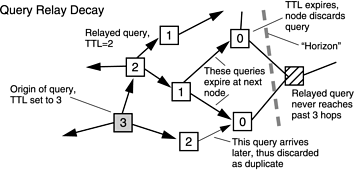
\includegraphics[width=0.7\textwidth]{src/img/p2p-systems/gnutella}
  \caption{Gnutella Architecture}
  \label{fig:p2p-systems:gnutella}
\end{figure}

Rețele P2P atomistice precum Gnutella sunt foarte dinamice și nu dispun de
liste de adrese centrale. Din punct de vedere pragmatic, totuși, este nevoie
de o listă de bootstrap pentru descoperirea inițială.

Efectul de "orizont" ține de segmentarea virtuală inerentă a rețelei, o
decizie de proiectare care limitează contorul de noduri la circa 15.000 pe
gNet, noduri vizibile de la un alt nod. Nodurile continuă să intre și să
părăsească rețeaua influențând astfel nodurile care pot fi atinse. Motivul
principal al apariției efectului de orizont este acela că mesajele au un
contor time-to-live (TTL). În mod tipic, valoarea TTL este configurată între 5
și 7 și este decrementată cu fiecare nod prin care mesajul trece. Un alt
contor monitorizează numărul de hopuri. Valorile TTL-ului și a numărului de
conexiuni de noduri, împreună cu capacitatea și lățimea de bandă a unui nod,
se combină pentru a determina performanța și stabilitatea rețelei. Unii
clienți permit utilizatorului ajustarea manuală a TTL-ului și a numărului de
noduri active, reușind astfel întrucâtva extinderea orizontului.

În tabelul de mai jos se poate observa evoluția orizontului (numărul de noduri
care pot fi atinse) raportat la valoarea câmpului TTL și a numărului de noduri
cu care are fiecare nod legătură:

\todo{tabel}

%TTL=2
%TTL=3
%TTL=4
%TTL=5
%TTL=6
%TTL=7
%N=2
%4
%6
%8
%10
%12
%14
%N=3
%9
%21
%45
%93
%189
%381
%N=4
%16
%52
%160
%484
%1456
%4372
%N=5
%25
%105
%425
%1705
%6825
%27305
%N=6
%36
%186
%936
%4686
%23436
%117186
%N=7
%49
%301
%1813
%10885
%65317
%391909
%N=8
%64
%456
%3200
%22408
%156864
%1098056

\subsubsection{The Gnutella Protocol}

Protocolul Gnutella este corelat puternic cu protocolul HTTP din Internet.
Criteriul definitoriu este că toate nodurile au drepturi egale și că un nod
acționează simultan ca server și client, denumit servant. Gnutella este
open-source și protocolul este relativ simplu, specificațiile fiind prezente
în diverse locații de pe Web.

Protocolul Gnutella definește numai 5 descriptori (antete de mesaje) care să
implementeze funcționalitatea rețelei. Fiecare descriptor de mesaj este
definit de un antet de mesaj, ale cărui componente sunt prezentate în tabelul
de mai jos. Acest antet de mesaj este de asemnea simplu conținând numai 5
câmpuri.

\subsubsection{Connection and Discovery}

Clienții Gnutella comunică folosind implicit portul 6346 folosind HTTP/1.0
care îi imprimă o funcționalitate de minibrowser/miniserver. Stabilirea unei
conexiuni în rețea se realizează prin intermediul unei conexiuni TCP către un
nod existent căruia i se transmite mesajul:

\begin{verbatim}
GNUTELLA CONNECT/<protocol version string>\n\n
\end{verbatim}

Un servant care dorește să accepte conexiunea va răspunde cu:
\begin{verbatim}
GNUTELLA OK\n\n
\end{verbatim}

Orice alt răspuns indică faptul că acel nod nu dorește să accepte acea
conexiune.

Un client poate alege să respingă o conexiune pentru o varietate de motive. Un
client poate alege să mențină doar conexiunile existente și să oprească orice
alte cereri de conexiune. Pot exista limitări de sloturi de coneixune sau un
servant nu poate funcționa pe versiunea de protocol folosită și să refuze
conexiunea.

Nodurile deja conectate în rețea pot mapa adrese de nod active prin mesaje de
tip ping-pong de la alte noduri, dar protocolul Gnutella nu specifică o metodă
inițială de descoperire a nodurilor active înainte de a se realiza alăturarea.
La început se distribuie adrese de nod cvasi-permanente prin alte canale
manuale iar noii utilizatori le introduc în clienți până când o conexiune este
stabilită. În zilele noastre, achiziția adreselor de nod se realizează de
obicei automat, prin intermediul serviciilor de caching pe nume de stații
implementate pe anumite noduri "permanente" ale rețelei.

Clienții configurați astfel pot menține automat liste locale bazate pe astfel
de download-uri și le pot utiliza mai târziu din cache-ul local. O dată
conectați la un nod activ, clienții pot mapa alte noduri de la mesaje de tip
pong recepționate, după transmiterea de mesaje de tip ping în rețea. Ca
rezultat direct, clienții stabilesc conexiuni cu alte noduri. Mai jos este
prezentată o astfel de hartă de conexiuni rezultată în urma unor răspunsuri de
noduri, limitată la un hop count de 4.

Mesajele de tip ping-pong reprezintă o porțiune semnificativă din traficul de
rețea într-o rețea P2P cumulând circa două treimi sau trei sferturi din toate
mesajele prin oricare conexiune. Drept urmare, protocolul Gnutella recomandă
minimizarea numărului și frecvenței de pachete de tip ping transmise de orice
client.

\subsubsection{Search}

Fundamental pentru protocolul Gnutella este căutarea, implementată prin
intermediul mesajelor de tip Query. Metoda obișnuită de broadcast înseamnă că
fiecare servant care obține cererea și verifică validitatea ei, realizează o
intrare a identificatorului în tabela cache și transmite cererea mai departe
conexiunilor existente. După aceasta, aplicația realizează o căutare în
conținutul propriu.

În plus față de șirul de căutare, descriptorul mai începe cu un câmp care
specifică rata de transfer minimă pentru răspuns. Astfel se indică servanților
cu rate de transfer mici să nu se deranjeze să răspundă. Totuși vor continua
transmiterea cererii mai departe. Servanții care găsesc o potrivire a șirului
de căutare răspund cu un mesaj de tipul Query Hit. Mesajul conține informații
despre nod și despre modul în care se poate realiza conectarea. Mesajele de
tip QueryHit sunt transmise înapoi în rețea, dar antetul conține același
identificator de descriptor ca și cererea. Acest lucru permite clientului care
a inițiat conexiunea să identifice și să asocieze mesajele de tip QueryHit
primite cu cele ale mesajelor de tip Query inițiate.

Un exemplu de cerere de transfer inițiată de un client este următoarea:

\begin{verbatim}
GET /get/<File Index>/<File Name>/ HTTP/1.0\r\n
Connection: Keep-Alive\r\n
Range: bytes=0-\r\n
User-Agent: <Agent Identifier>\r\n
\r\n
\end{verbatim}

Dacă totul decurge bine, servantul destinație va răspunde cu un antet de
confirmare:

\begin{verbatim}
HTTP 200 OK\r\n  Server: <Agent Identifier>\r\n
Content-type: application/binary\r\n
Content-length: 4356789\r\n
\r\n
\end{verbatim}

Un răspuns corespunzător permite servantului care realizează cererea să
înceapă descărcarea. Utilizatorul va stabili dacă banda și fiabilitatea
nodului destinație sunt satisfăcătoare și dacă se merită începerea
transferului.

\subsubsection{Transfer}

Deși transferul de fișiere are loc direct între cele două capete și, drept
urmare, nu încarcă restul rețelei, se partajează lățimea de bandă cu alte
transferuri. În plus, lățimea de bandă pentru transfer poate fi micșorată din
client astfel încât upload-urile sunt limitate la o anumită valoare, în ciuda
unei lățimi de bandă mari. Nu este neobișnuit ca rata de transfer pentru o
resursă să fie inițial foarte mare, urmând să scadă la valori inacceptabile în
scurt timp.

Parametrul Range din mesaj implică abilitatea de a relua transferurile
întrerupte de la un offset dat, lucru suportat de cei mai mulți servanți.
Posibilitatea de reluare a transferurilor este esențială în rețelele care se
modifică rapid unde fiecare nod se poate deconecta după bunul plac.

În ziua de azi, clienții prezintă suport pentru transferul diferitelor
segmente de fișiere de la diferite noduri. Transferuri paralele de la
offset-uri diferite îmbunătățește eficiența și fiabilitatea transferurilor și
este adesea o tehnică implementată în protocoale avansate.

Atât în cazul reluării transferului, cât și în cazul mai multor noduri,
problema este identificarea corectă a surselor ca fiind copii ale aceluiași
fișier. O metodă simplă este deplasarea diferitelor fragmente cu o valoare
mică și verificarea acelui deplasament. În cazul reluării unui transfer la un
moment ulterior, clientul care recepționează trebuie să-și amintească adresa
nodului asociat acelui fișier. Altfel, ar fi forțat să realizeze o nouă
căutare care poate duce la lipsa unei copii identifice a acelui fișier, sau
lipsa fișierului pe de-a-ntregul.

\subsubsection{Scalability}

O rețea Gnutella exemplifică atât avantajele cât și dezavantajele unei
arhitecturi P2P atomistice, mai ales în contextul a ceea ce se cheamă
"Transient Web". La fel cum am fost martorii creșterii Internetului intră în
acțiune constrângerile de scalabilitate inerente ale arhitecturii de bază.

Instalarea și folosirea Gnutella în cadrul unei rețele interne nu este
dificilă. Sarcinile administrative se limitează la instalarea celor mai
adecvați clienți cu o listă de noduri acceptată. Există clienți care
furnizează opțiuni pentru crearea unui astfel de tip special de "subrețea".
Crearea unei rețele limitate nu este o problemă. Principalul risc al acestui
context este dacă un nod ar trebui să se conecteze în afara listei
prestabilite de noduri. O astfel de conectare ar face întreaga listă de noduri
accesibilă din exterior. Este nevoie doar de un singur client pentru a suprima
"închiderea rețelei" în absența unor măsuri de filtrare care să prevină astfel
de conexiuni.

Soluții pentru o mai bună securitate se introduc pe măsură ce tehnologia se
maturizează. Exemple sunt sistemele de încredere automată și de control al
reputației.

\subsubsection{Trust and Reputation}

Implementările P2P de bază sunt de obicei deschise și nu au nici o formă de
gestiune a încrederii. Orice calculator care folosește un protocol compatibil
și dorește să se conecteze în rețea este automat acceptat. Totuși, deschiderea
totală înseamnă în același timp că rețeaua este deshisă intruziunilor
aplicațiilor malițioase. Metode de atac cunoscute sunt ping flooding, request
flooding, mesaje de găsit false, atacuri de tip denial of service pe nodurile
descoperite.

Configurările care să blocheze conexiunile bazate pe criterii specificate de
utilizator sunt disponibile pe toți clienții, dar comportamentul implicit este
să nu se filtreze nimic. Totuși, deschiderea inițială se schimbă și din ce în
ce mai mulți clienți încep să reconfigureze specificațiile implicite cu
configurații mai puțin permisive. Filtre tipice includ închiderea conexiunii
cu noduri care nu partajează conținut sau care au conexiuni prea puține și, în
plus, specificarea unor adrese IP care să fie blocate.

În ultima vreme, există un curent din ce în ce mai important care să
implementeze caracteristici mai sofisticate, lucru vizibil în implementările
inovative actuale. Noile forme de gestiune a conectivității aplicațiilor P2P
includ diverse forme de control a încrederii și reputației, semnături digitale
și criptare. Dorința este ca rețeaua să fie cât mai fiabilă și robustă fără ca
măsurile suplimentare de securitate să împiedice utilizatorii legitimi.
Totuși, dezvoltatorii P2P doresc de asemenea să evite administrarea centrală
și filtrarea care sunt caracteristici unor soluții orientate în jurul unui
server (server-centric).

\subsection{FastTrack}

Una din aplicațiile mai recente și inovative în arhitecturile peer-to-peer
este rețeaua FastTrack. FastTrack a sosit ca o soluție la problemele avute de
Napster și Gnutella. Rețeaua FastTrack este prin natura sa o arhitectură
hibridă, care, după cum s-a menționat și anterior, este o intersectare a două
sau mai multe topologii de rețea de bază. În cazul FastTrack este vorba de o
intersectare între topologiile centralizate și cele descentralizate.
Protocolul FastTrack

Protocolul FastTrack este o arhitectură proprietară, drepturile de utilizare a
rețelei trebuind a fi obținute de la compania Sherman Networks. Drept urmare
se cunosc foarte puține lucruri despre protocolul actual utilizat. Au fost
create mai multe încercări pentru a înțelege protocolul FastTrack (reverse
engineer). Cea mai cunoscută este proiectul giFT, care a fost foarte aproape
de "spargerea" protocolului. FastTrack a reacționat prin schimbarea criptării
folosite astfel încât este practic imposibil să mai fie dedus protocolul. Cu
toate acestea, efortul depus de proiectul giFT a fost suficient pentru a
permite definirea modului principal de funcționare a protocolului.

Tehnologia FastTrack folosește două niveluri de control în cadrul rețelelor
sale, așa cum reiese și din Figure~\ref{fig:p2p-systems:fasttrack}. Primul
nivel este format din clustere de noduri obișnuite care sunt conectate la
SuperNoduri (sisteme obișnuite care dispun de conexiuni de mare viteză). După
cum s-a discutat și anterior, acest tip de conexiune este similară topologiei
centralizate. Al doilea nivel este constituit din SuperNoduri conectate într-o
manieră descentralizată.

\begin{figure}
  \centering
  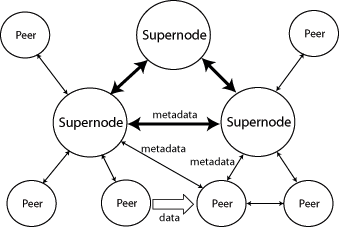
\includegraphics[width=0.5\textwidth]{src/img/p2p-systems/fasttrack}
  \caption{FastTrack Architecture}
  \label{fig:p2p-systems:fasttrack}
\end{figure}

Numărul de noduri definite ca SuperNoduri poate varia de la zeci la sute.
Acest lucru se datorează faptului că SuperNodurile sunt noduri obișnuite care
pot intra sau părăsi rețeaua după bunul plac. Drept urmare, rețeaua este
dinamică și într-o permanentă schimbare. Pentru a asigura disponibilitatea
constantă a rețelei este necesară prezența câtorva noduri care să monitorizeze
rețeaua. Astfel de noduri sunt denumite noduri de pornire (bootstrap nodes) și
trebuie să fie permanent activ (online). Când un client FastTrack (spre
exemplu, Kazaa), este pornit pe un nod, va contacta în primă fază nodul de
pornire. În continuare, nodul de pornire va determina dacă acel nod poate fi
considerat un SuperNod. Dacă da, atunci îi vor fi furnizate o parte (poate
chiar toate) din adresele IP ale celorlalte SuperNoduri. Dacă este clasificat
ca nod obișnuit atunci nodul de pornire îi va răspunde prin furnizarea adresei
IP a unuia dintre SuperNoduri.

Anumiți clienți precum Kazaa folosesc o metodă denumită sistem de reputație.
Reputația este asociată fiecărui utilizator și este reflectată de nivelul de
participare (o valoarea între 0 și 1000) în cadrul rețelei. Cu cât un
utilizator stă conectat mai mult timp, cu atât nivelul de participare este mai
mare, deci va fi favorizat în politicile de prioritate și va primi servicii
mai bune. Această măsură are scopul de a încuraja utilizatorii să partajeze
fișiere și să reducă numărul de "clienți pasageri" din rețea.

Descoperirea resurselor este îndeplinită prin intermediul difuzării între
SuperNoduri. Când un nod din cel de-al doilea nivel realizează o cerere este
dirijat către SuperNodul asociat care va difuza cererea celorlalte SuperNoduri
cu care este conectate. Difuzarea este reluată până când valoarea TTL-ului
atinge 0. Acest lucru furnizează clienților FastTrack o mai mare acoperire și
rezultate mai bune ale căutării. Un dezavantaj este metoda de difuzare care
poate duce la consumarea unei cantități importante de bandă în cazul
transferurilor între SuperNoduri. Totuși, această problemă nu este la fel
serioasă în cazul Kazaa ca în cazul Gnutella și datorită conexiunilor rapide
de care dispun SuperNodurile.

Fiecare SuperNod care a primit o cerere realizează o căutare în baza de date
de indexuri. Această bază de date conține informații despre toate fișierele
partajate de nodurile conectate. În momentul în care se găsește o potrivire se
transmite un reply către nodul original pe aceeași cale pe care a fost trimisă
cererea. Metoda este asemănătoare propagării răspunsului în rețeaua Gnutella.
Cu toate acestea, problema pierderii pachetelor nu este la fel de gravă ca în
cazul Gnutella. La Gnutella, backbone-ul rețelei este alcătuit din noduri care
se conectează sau se deconectează la rețea după bunul plac. În cazul
FastTrack, backbone-ul rețelei este alcătuit din noduri cu conexiuni de mare
viteză la rețea (SuperNoduri) și, drept urmare, căile de întoarcere pot fi
considerate mai sigure.

\subsection{eDonkey Network}

Rețeaua eDonkey este un sistem de partajare a fișierelor P2P centralizat. Un
set de servere centrale mențin informații de căutare despre diferitele fișiere
partajate de nodurile rețelei, urmând ca transferul efectiv de fișiere să aibă
loc direct între noduri.

Protocolul original eD2k nu a fost documentat formal. Totuși, ținând cont că
majoritatea clienților de astăzi (*Mule) sunt open-source se poate spune că
specificația formală pentru rețeaua eDonkey este modul în care clientul eMule
și serverul eserver interacționează. Prin rularea unui server eDonkey pe un
sistem conectat la Internet, orice utilizator poate adăuga un server în rețea.
Clienții își actualizează frecvent lista de servere pentru că adresele lor
continuă să se schimbe.

Fișierele din rețeaua eDonkey sunt identificate unic cu ajutorul unui rezumat
MD4. Acest lucru înseamnă că fișierele cu conținut identic dar nume diferite
sunt aceleași. Fișierele sunt împărțite în "calupuri" de câte 9.728.000 (9500
x 1024) octeți plus un calup rezidual. Pentru fiecare calup se calculează o
sumă de control MD4 de 128 de biți. În acest fel o eroare se detectează o
eroare de transmisie și coruperea este realizată numai la nivel de bloc, nu și
la nivel de fișier. În plus, calupurile valide descărcate cu succes sunt
disponibile pentru partajare înainte ca restul fișierul să fi fost descărcat,
la fel ca în cazul protocolului BitTorrent.

Inițial, protocolul eDonkey folosea un set de servere folosite de utilizatori
care donau lățimea de bandă necesară și overhead-ul de procesare și spațiu de
disc. Astfel de servere sunt subiectul traficului intens și, drept consecință,
sunt mai vulnerabile la atacuri.

Rezultatul a fost dezvoltarea Overnet de către MetaMachine, dezvoltatorul
inițial al clientului eDonkey, și Kademlia de către proiectul eMule.

Kademlia este versiunea fără server a rețelei eDonkey, asemănătoare cu
Gnutella. Spre deosebire de Gnutella, însă, Kademlia folosește tabele hash
distribuite (DHT – Distributed Hash Tables) pentru a stoca informații despre
localizarea fișierelor în cadrul rețelei. Astfel, dacă la Gnutella, căutarea
unui fișier se realiza prin "inundarea" rețelei cu mesaje de tipul Query, în
cazul Kademlia căutarea se realizează pe baza unei funcții hash care permite
identificarea nodurilor unde s-a reținut informația de localizare a fișierului
dorit. Informația de localizare este stocată în cadrul mai multor noduri
pentru a permite intrarea în sistem sau părăsirea sistemului fără a pierde
informațiile de localizare.

Intrarea în rețea se realizează, ca și în cazul Gnutella, prin intermediul
unui nod de bootstrap cunoscut de la început de clientul Kademlia.

\subsection{DirectConnect}

DirectConnect este un protocol de partajare de fișiere de tip P2P centralizat.
Protocolul DirectConnect are o arhitectură asemănătoare cu Napster. Dar, dacă
în cazul Napster era vorba de un singur server central (și deci de un unic
punct de cădere), în cazul DirectConnect există servere dedicate denumite
hub-uri unde se pot conecta clienții.

Protocolul DirectConnect este un protocol text, comenzile și informațiile
fiind trimise în clar, fără a fi criptate. Întrucât clienții se conectează la
o sursă centrală de distribuție (hub) a informației, hub-ul trebuie să dețină
o lățime de bandă substanțială.

Nu există o specificație oficială a protocolului. Acest lucru înseamnă că
fiecare client sau hub a obținut informația referitoare la modul de
funcționare prin spargerea protocolului inițial (reverse engineering).

Partea P2P a protocolului se bazează, la fel ca și în cazul eDonkey, pe
conceptul de slot, un număr care denotă număr de utilizatori care pot descărca
simultan fișiere de la utilizatorul curent. Aceste sloturi sunt controlate de
client. Download-urile folosesc TCP iar cererile active folosesc UDP. Un
client se poate găsi în două stări: activă sau pasivă. Clienții în starea
activă pot descărca de la oricine altcineva din rețea. Clienții în starea
pasivă pot descărca numai de la cei activi.

Hub-urile dețin informații despre clienți ca și abilități de căutare și chat.
Transferul de fișiere are loc direct între clienți, așa cum este comun într-un
sistem P2P. Multe hub-uri au cerințe raportate la numărul total de fișiere pe
care membrii săi le pot partaja și restricții referitoare la conținutul și
calitatea fișierelor partajate. De asemenea, un hub poate alege anumiți
utilizatori ca operatori pentru a susține anumite reguli pe care hub-ul nu le
poate susține de unul singur. O problemă a hub-urilor DirectConnect este aceea
a scalabilității, natura server-centrică a arhitecturii împiedicând acest
lucru.

\subsection{Instant Messaging. Jabber/XMPP}

Una din cele mai folosite forme de aplicații P2P este, în ziua de azi,
mesageria instantă (instant messaging). La începutul Internet-ului, serviciul
de poștă electronică (e-mail) era inerent peer-to-peer. Mesajul era transmis
prin realizarea unei conexiuni de la un terminal al unui utilizator la un alt
terminal. Totuși, de-a lungul timpului, comunicația între utilizatori a
devenit una indirectă. Cele mai multe calculatoare personale nu suportau
versiunile de protocol folosite în comunicație, folosind servere dedicate
(MTA) pentru transmiterea mesajelor.

O problemă a serviciului de e-mail era faptul că nu acționa ca un serviciu în
timp real. Mesajele puteau fi pierdute sau întârziate. Consecința a fost
apariția aplicațiilor de chat care permiteau comunicația în timp real. La
început au apărut aplicații de chat cu comunicația intermediată de servere
(server-relayed chat). Un exemplu este IRC (Internet Relay Chat). Acest tip de
aplicație nu este peer-to-peer. Cu toate acestea, IRC poate fi văzut ca un
precursor al P2P de tip utilizator întrucât permite nodurilor să se descopere
și să inițieze contact direct folosind alte tehnologii ale clientului.

În mod confuz, termenul "chat" este folosit atât pentru retransmitere prin
difuzare către mai mulți utilizatori (broadcast relay) cât și pentru mesaje
private transmise de-a lungul unei conexiuni punct la punct. Un grup separat
de aplicații sunt dedicate celei de-a doua categorii consemnând ascensiunea
mesageriei instante. Cu alte cuvinte, denumirea de "instant messaging" se
referă la versiuni de chat care implică existența unei conectivități între
nodurile comunicante.

Principalul scop al Jabber/XMPP (eXtensible Messaging and Presence Protocol)
este o "tehnologie de conversație" pentru P2P în sensul general, incluzând nu
numai comunicație utilizator-utilizator dar și utilizator-aplicație sau
aplicație-aplicație. Jabber a evoluat astfel ca un proiect care să aducă la un
loc diverse aplicații în urma deciziei unui număr de utilizatori de a crea o
arhitectură P2P deschisă și distribuită drept bază pentru muncă specializată.
Proiectarea a presupus alegerea XML ca un mod consistent de încapsulare a
informației, indiferent de aplicație, permițând în același timp extensii.
Protocoalele de aplicație sunt implementate transparent în XML și translatate
în formatul nativ după cum se dorește.

Unele din proiectele dezvoltate în cadrul Jabber sunt:
\begin{itemize}
  \item gateway pentru majoritatea protocoalelor de mesagerie instantă
  \item biblioteci pentru aproape toate limbajele de programare
  \item un server open-source modular plus clienți pentru orice platformă
  \item un număr de servere specializate precum traducerile de limbaje
\end{itemize}

Un accent aparte este atribuit comunicației utilizator-aplicație și abordării
de proiectare care facilitează toate formele de comunicație P2P. Prima
aplicație practică a tehnologiei Jabber este un sistem mesageria instantă care
ține cont de securitate, ușurință în folosire, acces de oriunde folosind orice
tip de dispozitiv și interoperabilitate cu servicii Web, de mesagerie instantă
sau telefonie.

Central arhitecturii deschise este faptul că toată comunicația are loc
folosind formatul XML, permițând Jabber să funcționeze atât ca un serviciu de
stocare cât și ca unul de schimb. Metainformația și structura sunt în mod
similar definite în XML și s-au stabilit seturi de taguri care să descrie
fișiere de tip document, audio, video etc. Deși Jabber poate fi folosit cu mai
multe scopuri, implementarea sa cea mai comună este un client IM.

\subsubsection{Infrastructure}

Modelul de inspirație pentru Jabber este serviciul de e-mail al Internet-ului:
o rețea distribuită de servere care folosesc un protocol obișnuit, la care se
pot conecta mai mulți clienți pentru a transmite sau a recepționa mesaje. În
cazul Jabber, acest lucru poate însemnă și alte servicii. Principala diferență
funcțională dintre Jabber și e-mail este aceea a incorporării prezenței și
apropierea de comunicația în timp real, spre deosebire de sistemul "stochează
și transmite" al serviciului de e-mail.

Serverele sunt total independente unul față de celălalt și mențin o listă
proprie de utilizatori și servicii. Mesajele sunt transferate într-o rețea P2P
atomistică. Orice număr de servere Jabber pot forma o rețea. Un utilizator
particular este asociat cu un server specific și o identitate care apare ca o
adresă de e-mail (george@jabber.org).  Această identitate este asociată unui
proces de înregistrare sau în timpul unei configurări administrative a
serverului.

Pe formatul amintit mai sus al identității, o aplicație Jabber poate expune
date interne accesului public. Un URI extern ar putea avea formatul:
\texttt{jabber://user@server/resource/data}.

\subsubsection{Jabber Clients and Servers}

Pe de o parte, Jabber este o arhitectură preponderent client-server. Clienții
se conectează la un server Jabber înainte de orice transfer P2P. De asemenea,
mesajele de chat Jabber sunt dirijate prin intermediul serverului. Fiecare
sesiune creează un "flux de comunicație XML" către serverul contactat, flux
care durează cât o sesiune online.

Conexiunile directe între noduri sunt definite ca specifice aplicației: sunt
perfect posibile, dar trebuie întâi negociate în contextul client-server. O
parte din deciziile de proiectare ale Jabber a fost mutarea unei astfel de
complexități către o componentă de tip server. Dezvoltatorii pot astfel crea
clienți foarte ușor și este ușor pentru administratorii de sistem să adauge o
nouă funcționalitate fără actualizări masive ale aplicațiilor tip client.
Nucleul serverului Jabber este relativ redus, astfel că fiecare sistem ar
putea avea propriul server Jabber integrat, ceea ce ar fi echivalent cu un
sistem P2P atomistic din punct de vedere al utilizatorului.

Folosirea XML este un punct important al arhitecturii pentru că marcajele XML
pot exprima orice informație structurată. Toate componentele Jabber trebuie să
poată comunica folosind XML, chiar și atunci când se transferă informații ce
ar putea folosi extern alte protocoale.

\subsubsection{The Jabber Protocol}

Mesajele specifice Jabber sunt conținute în trei tipuri mari de mesaje XML:
message, presence și info/query (iq). Structura și sintaxa sunt foarte simple
și în format text. Un exemplu poate fi:

\begin{verbatim}
<message to='user@server' type='chat'>
    <body>The actual text of the message.</body>  
</message>
\end{verbatim}

Un câmp from este adăugat de server în momentul transmiterii mesajului. Tipul
este opțional și se reduce, implicit, la mesaj obișnuit. Tipul 'chat' înseamnă
că acest client afișează acest mesaj într-o fereastră de chat. Alte elemente
de mesaj sunt: html, subject, thread (pentru menținerea de informații despre
replici la mesaj), x (folosit pentru extensii). Folosirea x înseamnă că se va
declara un spațiu de nume separat cu funcționalitate specializată.

\subsection{P2P Collaborative Spaces. JXTA}

Multe dintre aspectele inovative ale Internet-ului au evoluat în ansamblu ca
un rezultat direct sau indirect al dorinței oamenilor de a colabora
independent de locația acestora. Tehnologiile peer sunt naturale pentru forme
de colaborare informală în mai multe moduri și încurajează formarea unor
astfel de grupuri colaborative de persoane. În absența prezenței fizice mulți
oameni au nevoie să lucreze împreună și este vital să nu existe bariere în
calea comunicației efective. Grupările P2P informale sunt cel mai bun mecanism
de lucru.

Mai mult, aceste grupări informale sunt folosite pe scară largă de foarte
mulți oameni, indiferent de structurile formale care pot fi impuse central.
Tendința este atât de intensă încât oamenii nu-și dau seama că exact acest
lucru se întâmplă. Când vor fi întrebați, vor spune că lucrează conform
metodologiei de lucru dintr-o structură ierarhică. Cu toate acestea, studii
efectuate de persoane externe grupului arată o succesiune rapidă de contacte
în format P2P.

Proiectul JXTA, prescurtare de la juxtapunere, adică unul lângă altul, este o
inițiativă a Sun Microsystems care încearcă să integreze tehnologiile P2P ca
utilitare complementare și distribuite în Internet și în sistemele de calcul.
Platforma de bază este o arhitectură de rețea complet descentralizată. Totuși,
atât servicii centralizate cât și descentralizate pot fi dezvoltate peste
această platformă.

\subsubsection{JXTA Architecture}

Intenția arhitecturii JXTA este ca entități de rețea arbitrare să fie capabile
să descopere alte entități de rețea și să colaboreze cu acestea în moduri
conform cu aplicațiile. Nu este nevoie de nici un suport de platformă
particular a oricăruia dintre participanți dar prezintă forma și conținutul
mesajelor de descoperire schimbate în cadrul rețelei.

Arhitectura este descrisă folosind trei niveluri:

\begin{itemize}
  \item nivelul aplicație: suportă implementarea de aplicații integrate precum
  partajarea fișierelor, partajarea resurselor și spațiul de stocare
  distribuit;
  \item nivelul servicii: furnizează interceptări de API pentru servicii de
  rețea generice, folosite în mod obișnuit de aplicații P2P; exemple includ
  căutare, partajare, caracteristici de securitate;
  \item nivelul pricipal (core layer) care implementează protocoalele și
  componentele esențiale pentru o rețea P2P; acest nivel include descoperirea
  nodurilor, un nivel de transport cu specificații de lucru cu firewall-uri și
  aspecte de securitate.
\end{itemize}

Întreaga proiectare este una modulară permițând dezvoltatorilor să aleagă
serviciile sau aplicațiile care se potrivesc cu nevoile lor. Nucleul comun
permite serviciilor dezvoltate să fie interoperabile și aplicațiile
particulare să se amestece și să se potrivească cu caracteristicile dorite
folosind module existente sau noi.

\subsubsection{Groups and Nodes}

În contextul JXTA, nodurile sunt definite ca orice dispozitiv care cunoaște
cel puțin o parte din protocoalele proiectului JXTA. Definiția poate include
un număr mare de dispozitive de la servere, PC, PDA până la telefoane mobile
sau echipamente embedded. Singura cerință este ca nodurile să fie conectate la
un tip de rețea (IP, Bluetooth etc.)

Un grup este cuprins dintr-o colecție de noduri care s-au înțeles pe un set
comun de reguli de comunicație între acestea. Fiecare grup poate stabili
politicile proprii de membri, începând de la grupuri total deschise până la
grupuri foarte sigure și protejate.

În terminologia JXTA, obiectele Java folosite în transmisie care conțin și cod
și data se chemă codate (codat/codats).

\subsubsection{Security Model}

În centrul securității proiectul JXTA se găsesc scheme de criptare și
semnături de chei publice/chei private. Un astfel de sistem asigură securitate
puternică dacă se găsește într-un context de "încredere".

Modelul de încredere, denumit "P2P Web of Trust", este similar cu denumirea
"Web of Trust" a PGP folosită pentru securizarea mesajelor de e-mail și este
folosit pentru transferul de chei publice între membri. Fiecărui membru i se
asociază un anumit nivel de încredere, formal sau informal. Cheile care sunt
semnate de membrii de încredere capătă statut de încredere. O politică de grup
poate acorda anumitor membri autoritatea de semnare a cheilor publice ale
altor membri, în plus față de sarcinile de rutină precum autentificarea,
adăugarea sau eliminarea de membri.

Există clase de securitate pentru algoritmi obișnuiți (RSA, RC5, SHA-1).
Combinațiile de clase de securitate formează grupuri de implementare a
securității.

\subsubsection{Projects Using JXTA}

Pagina principală a proiectului JXTA (https://jxta.dev.java.net/) oferă
informații despre diversele platforme, servicii și aplicații.

Componentele principale ale JXTA sunt dezvoltate în cadrul unui număr de
proiecte separate: jxme (pentru platforme mobile), jxta-c, jxtaperl, jxtaruby,
platform (pentru Java SE), pocketjxta, security.

Serviciile de bază ale JXTA includ autentificarea, descoperirea și
managementul codatelor. Alte servicii includ denumirea, rutarea, căutarea și
indexarea codatelor. Câteva servicii sunt prezentate mai jos:

CMS: JXTA implementează un serviciu de gestiune a conținutului (Content
Management System) cu partajarea de-a lungul nodurilor unui grup. Aplicația
InstantP2P folosește serviciul CMS pentru a implementa căutarea, partajarea
comenzilor shell.

proiectul Edutella folosește o rețea P2P pentru a schimba resursele
educaționale între diversele universități. Viziunea este să furnizeze servicii
de metainformație necesare pentru a permite interoperabilitatea între
aplicații JXTA eterogene.

Proiectul JxtaVFS urmărește gestiunea fișierelor virtuale, reprezentând
fișiere dinamice mapate peste resurse aflate la distanță; este un mod de a
crea o hartă distribuită, ierarhică și autosusținută de resurse în cadrul
rețelei.

Proiectul Payment Project are scopul de implementare a unui protocol
EPocketCash pentru tranzacții financiare pentru JXTA, care permite tuturor
utilizatorilor să devină cumpăratori sau vânzători de pe același cont.

Proiectele de aplicație JXTA permit accesul interactiv la platforma P2P JXTA.
Multe dintre ele ocupă puțin spațiu.

JXTA Shell este un interpretor opțional în linia de comandă care permite
utilizatorilor și dezvoltatorilor să interacționeze cu platforma JXTA

Gnougat este un servant Gnutella implementat peste tehnologia JXTA.

Există un număr mare de proiecte aflate în dezvoltare. JXTA ar trebui să fie
văzută ca o platformă alternativă, descentralizată, P2P cu funționalitate
open-source care poate atinge sau depăși viziunea centralizată și proprietară
a platformei .NET.

\section{Content Distribution in Peer-to-Peer Systems}
\label{sec:p2p-systems:streaming}

O alternativă a partajării simple de conținut, în care fișierele
utilizatorilor sunt accesate conform deciziilor locale ale fiecărui nod din
rețeaua P2P este introduderea distribuirii spațiului de stocare în cadrul
rețelei. Cu alte cuvinte, conținutul agregat nu este suma fișierelor pe care
fiecare nod permite să fie partajate ci un conținut public accesibil întregii
rețele. Diverse metode de implementare a spațiului de stocare distribuit
furnizează moduri noi și puternice de gestiune a conținutului și
disponibilitații acestuia.

\subsection{Swarmcast}

O implementare ce se concentreaza in mod explicit pe distributia multimii
continutului divizat intr-o multitudine de parti este ceea ce numim Swarmcast.
Se bazeaza pe puterea serverului central de a administra o retea cu clienti
distribuiti.

Swarmcast este promovat ca un sistem de distributie de continut de mare viteza
pentru fisierele mari în locul unui sistem cu distributie de fisiere. Editorii
fisierelor cu continut foarte mare, cu multe solicitari asteptate, pot sa
distribuie eficient si fiabil aceste fisiere multor utilizatori cu costuri
mici pentru latimea de banda. Utilizatorii obseva ca pot descarca fisiere mari
repede si mai fiabil pentru ca tehnologia de swarming se adapteaza cererilor
privind alocarea spatiului de scara si mutiplicarea continutului aproape de
punctele de cerere.

Solutia oferită de Swarmcast are doua componente principale:

\begin{itemize}
  \item{Swarmcast Gateway este o parte comerciala a programului serverului.Ca
  efect, publica continutul ca parti unui număr de noduri si apoi distribuie
  fiecare cerere de descarcare primita de la utilizator catre nodurile
  disponibile sa serveasca aproape toate partile fisierului cerut.}
  \item{Swarmcast Client este programul pe care un utilizator poate sa il
  descarce gratuit. Il instaleaza pe propria masina pentru activarea
  descarcarii fisierelor swarmcast.}
\end{itemize}

Tehnologia poate fi facuta sa lucreze si cu alte aplicatii, cum ar fi manageri
de descarcare, software updaters si cu aplicatii de distributie de fisiere.

\subsubsection{SwarmCast at Work}

Swarmcast se bazeaza pe modul in care clientii de Web solicita fisiere de la
un server HTTP Web. Ofera o arhitectura centrată pe conținut, unde continutul
in mod original este publicat si apartine serverului central. Fiecarui fisier
i se aloca o cheie (hashed-key SHA-1), care asigura integritatea datelor si
independenta numelui si permite autentificarea si functionalitati private. 

Cerintele pentru un transfer al datelor rapid si fiabil catre multi
utilizatori sunt indreptate in doua directii: oferind multe cai P2P pentru a
reduce banda pe fiecare cale, si o codare redundanta avansata a partilor
transferate. Se incearca in mod agresiv impingerea continutului catre retelele
locale de perechi interesate, eliberand banda centrala si minimizand caile de
date pentru majoritatea nodurilor. Tehnologia Swarmcast in implementarea sa de
baza nu mentine o retea P2P durabila. In schimb presupune un server central
normal ca ultima sursa pentru intregul continut. Utilizatorii stiu doar de
aceasta sursa centrala, si poate fi in locuri diferite, sau poate reflectata
in moduri traditionale.

Utilizatorii parcurg si cer anumite fisiere prin intermediul clientilor
acestora, care se conecteaza la server prin gateway pentru a descarca
fisierele. Apoi serverul central permite descarcarea. Fisierul este impartit
apoi in pachete codate indentificabile de gateway si trimise clientilor.
Cerintele unui anumit fisier nu sunt cu mult diferite fata de descarcarile
client-server normale.

\subsubsection{Bandwidth Shaping}

Lucrurile devin mai interesante cand mai multi utilizatori fac cerere pentru
acelasi fisier. Atunci gateway-ul cicleaza prin pachetele fisierului
respectiv, distribuind la intamplare aceste pachete  clientilor. Astfel
fiecare nod primeste o portiune a pachetului original, dar si programul
clientului este constient de alte noduri care primesc pachete ale aceluiasi
fisier. In timp nodurile primesc pachete și le redifuzeaza unul altuia.
Pachetele fisierelor sunt schimbate repede intre nodurile din rețea, la
capacitatea maxima a clientului si a retelei locale, fara a fi constranse de
banda serverului.

Reamintim ca distributia pachetelor a fost aleatorizata de gateway. Nodurile
verifica pachetele primite pentru a vedea daca reconstructia fisierului se
face corect. Distributia gateway-ului face ca pachetele schimbate intre noduri
sa ajute la descarcare. Schema de codare asigura ca pachetele pot fi primite
in orice ordine, si cand au fost primite indeajuns de multe pachete
folositoare, fisierul este decodat.

De indata ce nodul a  terminat de reasamblat fisierul cerut, poate sa
paraseasca reteaua. Acest lucru este optional oricum, si utilizatorii isi pot
pastra calculatoarele ca parte a retelei pentru un timp, dupa ce au terminat
de descarcat fisierele. Mentinandu-se in retea, acesti utilizatori ajuta pe
altii la descarcarea mai rapida a  aceluiasi continut , deoarece copiile
complete ale pachetelor fisierelor descarcate sunt disponibile pentru
redifuzare imediat.

In cazurile in care sunt multe cereri pentru aceleasi fisiere, si astfel multe
noduri ce formeaza reteaua de descarcare, crescand nuamarului de noduri ce pot
sa inlocuiasca parti ale aceluasi continut, vor satura capacitatea de
descarcare a unui singur client. Acum, de indata ce a oferit o copie completa
a continutului, serverul central nu mai trebuie sa raspunda la cereri pentru
ca acestea sunt duse la bun sfarsit de retea.

\subsubsection{Load Balancing}

Dinamizarea retelei este baza pentru adaptarea la scalabilitate si incarcare
in tehnologia Swarmcast. De indata de numarul cererilor creste, creste si
disponibilitatea de distributie a continutului. Presupunand ca sunt destui
clienti, ei pot descarca eventual de la surse paralele la rata de varf a
fiecaruia. Intre timp serverul este liber sa trateze cereri pentru alt
continut. Noi retele se formeaza automat in jurul nodurilor ce descarca alt
continut, la fel neincarcand serverul. O defectiune are loc daca numarul
clientilor din retea va scadea, cand cand ei nu mai pot satisface cererile,
gateway-ul pasand inca o data cererile catre severul central.

Un efect secundar al acestei solutii este ca acelasi server de continut poate
fi folosit pentru a duce la bun sfarsit in acelasi timp si cererile
utilizatorilor de folosesc Swarmcast, si ale celor care nu folosesc Swarmcast.
Primii clienti se conecteaza la gateway si culeg beneficiile permise de
acesta, in timp ce ultimii se conecteaza direct la serverul principal ca si
mai inainte. In aceasta privinta, tehnologia Swarmcast este o tehnologie punct
la punct ce adauga inca un canal de distributie care descarca serverul
central.Ca efect , distributia volumului este mai eficienta chiar si pentru
clientii ce folosesc tehnologii mai vechi, deoarece clientii noi nu vor
concura pentru aceeasi banda.

\subsubsection{Redundant Encoding}

A doua caracteristica ca importanta implementata in aceasta tehnologie este
folosirea codarii FEC (Forward Error Correction) pentru cresterea fiabilitatii
in momentul transferului. Codarea are particularitatea de a face tehnologia
Swarmcast independenta de protocolul de nivel retea. 	Multe aplicatii ale
retelelor folosesc o forma de codare FEC pentru a oferi toleranta la erori.
Figura de mai jos arata principiul de codare bloc folosit in tehnologia
Swarmcast, denumit RFEC (Redundant FEC). Recuperarea este posibila chiar si
cand s-au pierdut un numar mare de pachete in timpul transferului. Nu conteaza
ce pachete sunt primite, numai sa ajunga un numar minim de pachete decodate
corect fara sa conteze ordinea in care au ajuns.

Chiar daca redundanta introdusa de o asemenea codare ar creste  cererile de
latime de  banda pentru aceasi capacitate, acest lucru nu este la fel in
practica. Aceasta metoda permite un protocol de transfer cu mai putine mesaje
intre noduri. Transferul fiabil fara redundanata si corectia erorilor duc la
necesitatea ca fiecare pachet sa fie confirmat, si toate sa fie primite
corect. Daca vreun pachet este pierdut sau eronat, clientul trebuie sa ceara
retransmiterea acestuia, chiar de multe ori daca reteaua este incarcata. Cu
cat umarul cererilor de retransmisie creste reteaua se va supraincaraca si nu
lucra la parametri normali.

Printr-o analiza bazata pe situatia de multicast a unei singure surse se poate
arata castigul de latime de banda prin folosirea codarii FEC. Presupunem ca
10.000 de utilizatori primesc o transmisie de multicast si ca rata medie de
pierdere a pachetelor este de 10 procente. La protocoalele de transport
fiabile (cum ar fi TCP-ul), toate pachetele sunt difuzate trimise si retrimise
pana cand toti receptorii au confirmat fiecare pachet. Presupunand o pierdere
independenta a unor pachete ale utilizatorilor din acest exemplu, fiecare
pachet ca ajunge sa fie transmis in medie de cinci ori.

Comparam aceasta situatie de consum de latime de banda cu o situatie in care
transmisia este arbitrar divizata in 100 000 de mii de pachete si este folosit
un cod FEC pentru a adauga 25 000 de mii de pachete redundante la transmisie.
Pachetele sunt trimise toate o data. Apoi este suficient ca utilizatorii sa nu
piarda mai mult de 25 000 de mii de pachete pentru a putea decoda fiabil
mesajul.

Sa expunem cele doua circumstante fundamentaledespre transferul pachetelor cu
codare FEC:
\begin{itemize}
  \item receptia pachetelor nu trebuie sa fie confirmata
  \item nu sunt necesare retransmiteri
\end{itemize}

Totalul latimii de banda utilizata la aceeasi rata de pierderi ca in situatia
originala de retransmitere este aici de patru ori mai mica, fara a lua in
considerare intarzierea care poate fi minimizata folodind  un protocol mult
mai simplu. Exemplul de multicast a fost bazat pe codarea FEC ideala, care in
implementarea practica s-a dovedit a fi prea lenta. O schema de codare IFEC
("irregular" FEC) inventata de catre Michael Luby si Michael Mitzenmacher
pentru a permite implementari mai rapide.

Codul IFEC permite ca decodarea si codarea sa aiba loc intr-un timp
proportional cu lungimea codarii, multiplicat cu o constanta(valoarea tipica
5) ce este independenta de numarul de pachete redundante.Timpii de codare si
decodare ai codurilor FEC standard prin contrast sunt proportionali cu
lungimea de codare inmultita cu numarul pachetelor redundante - în mod evident
un factor mai mare pentru toate fisierele.

In general, algoritmul IFEC poate fi proiectat pentru orice formă de compromis
ales intre limitele fiabilitatii  si dimensiunea/timpul unei intarzieri
acceptabile.Timpii caracteristici decodarii IFEC pentru fisiere cu dimensiuni
de ordinul megaoctetilor este mai mic de o secunda in momentul de fata.

Ceea ce tehnologia Swarmcast nu incearca sa adreseze este dependenta de
serverul central de continut. Acest lucru aseaza tehnologia la marginea
acestui studiu P2P, deoarece clientii pereche, din punctul de vedere al
utilizatorului, sunt in intregime destinatarii continutului central publicat,
si utilizatorii vad numai acest server, nu perechile.

\section{BitTorrent}
\label{sec:p2p-systems:bittorrent}

O analiză întreprinsă de cercetătorii de la Xerox Palo Alto Research Center
indică faptul că circa 50\% dintre fișierele partajate sunt stocate pe 1\%
dintre noduri. Circa 70\% din utilizatorii Gnutella nu partajează fișiere cu
alți utilizatori. Cu alte cuvinte, ei doar "descarcă" resurse și sunt denumiți
"freeloaders" sau "freeriders".

Dacă o rețea deține un număr mare de freeloaders, atunci se pierde scopul
repartizării încărcării într-o rețea P2P. Când un nod partajează un fișier
popular cu alte noduri în cadrul rețelei P2P va atrage un volum mare de
trafic. Acest nod trebuie să plătească mai multă bandă pentru mai mulți
clienți.

BitTorrent este un nou protocol folosit pentru a rezolva această problemă.
Ideea din spatele protocolului este simplă: nodul care joacă rolul serverului
împarte fișierul în mai multe sub-fișiere. Dacă fișierul este solicitat de mai
mulți clienți simultan fiecare client va obține o parte diferită din fișier.
În momentul în care un client obține un sub-fișier complet va permite altor
clienți să descarce acest subfișier în timp ce el va continua descărcarea
celui de-al doilea subfișier. Cu alte cuvinte, nodul va acționa simultan ca
server și client după recepționarea primului subfișier. Procesul continuă până
când download-ul este complet.

Protocolul BitTorrent este foarte potrivit pentru descărcarea fișierelor de
dimensiune mare unde procesul de descărcare este mai lung. Aceasta are drept
consecință existența mai multor servere pentru o perioadă mai lungă de timp.
Mai mulți participanți nu vor descrește performanța întregii rețele pentru că
încărcarea este distribuită. În mod evident performanța va fi îmbunătățită
pentru că nu există o metodă de a dezactiva funcția de upload a unei aplicații
BitTorrent pe măsură ce nodul realizează download.

Figure~\ref{fig:p2p-systems:bittorrent} se prezintă o diagramă schematică.
Serverul are 4 subfișiere. Fiecare client obține un subfișier de la server la
un moment dat.  După cum se observă, clientul 1 obține aceste 4 subfișiere de
la sisteme de calcul diferite. Modul în care subfișierele ajung la client pot
să nu respecte ordinea inițială. Algoritmul BitTorrent va încerca maximizarea
numărului de subfișiere disponibile pentru download la un moment dat.

\begin{figure}
  \centering
  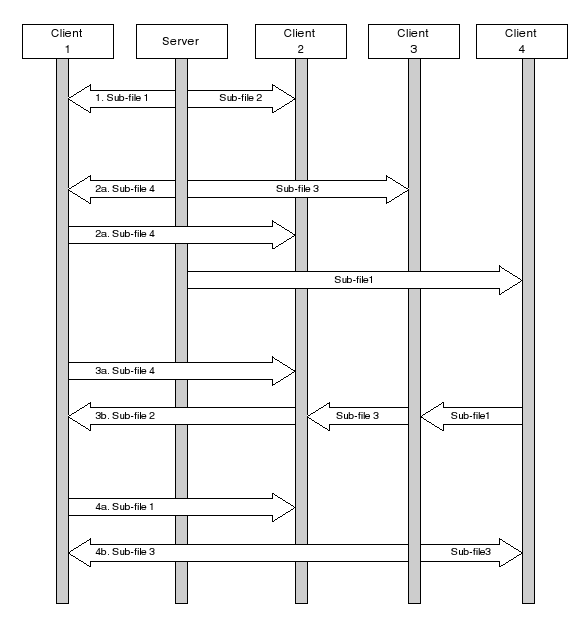
\includegraphics[width=0.4\textwidth]{src/img/p2p-systems/bittorrent}
  \caption{BitTorrent File Sharing}
  \label{fig:p2p-systems:bittorrent}
\end{figure}

Pentru a descărca un fișier un utilizator folosește următorii pași:

\begin{itemize}
  \item instalează o aplicație BitTorrent
  \item navighează Web-ul
  \item găsește un fișier pe un server
  \item selectează locația unde să fie salvat fișierul
  \item așteaptă încheierea procesului
  \item instruiește programul să se închidă (procesul de upload continuă până
  când utilizatorul realizează acest pas)
\end{itemize}

Această metodă permite distribuirea fișierelor mari (precum fișierele video)
unui număr mare de sisteme de calcul într-un timp scurt. Există mai multe
aplicații ale acestei tehnologii. Spre exemplu, anumite portaluri furnizează
video în timp real clienților în timpul campionatului mondial de fotbal.
Totuși, portalurile nu au făcut față numărului mare de cererei de conexiune și
multe conexiuni nu au fost acceptate. Folosirea BitTorrent poate rezolva
astfel de probleme cu ușurință.

\todo{more on this}

\section{Issues in Peer-to-Peer Systems}
\label{sec:p2p-systems:issues}

\todo{issues}

%Viitorul rețelelor P2P
%
%Tehnologia de tip P2P promite să ofere fiecărui individ acces la servicii și
%conținut distribuit liber. Termenul liber nu înseamnă neapărat fără cost,
%fiind disponibile mai multe metode de plată în practică. Posesia individuală
%a conținutului și serviciilor înseamnă acces personal direct, libertate în
%utilizare și libertate în mișcare. La fel ca și în cazul posesiei de
%proprietate fizică, presupunerea este că individul poate delega drepturi
%suplimentare entităților în care are încredere.
%
%Viziunea P2P încapsulează, de asemenea, conceptul împuternicirii
%utilizatorului, care este o ambiție importantă de multe ori pierdută sub
%deviza "ușurinței în utilizare".
%
%Câteva dintre expresiile împuternicirii utilizatorului sunt aceste acțiuni:
%crearea de conținut și servicii și posibilitatea localizării lor pe orice
%dispozitiv disponibil
%accesarea resurselor și serviciilor cu orice dispozitiv disponibil indiferent
%de sursă, locație sau timp
%gestionarea propriului conținut și a serviciilor
%partajarea de conținut cu familia, cunoscuții și restul lumii
%menținerea confidențialității și integrității informațiilor personale și
%proprietare
%coordonarea livrării de servicii și conținut
%personalizarea prezentării, conținutului și serviciilor
%
%Internet2
%
%Internet2 este format în jurul unui consorțiu de 180 de universități care
%lucrează în parteneriat cu guvernul și industria și a fost fondat pentru
%dezvoltarea și utilizarea tehnologiilor și aplicațiilor de rețea avansate.
%Așa cum se menționează și pe site-ul web (http://www.internet2.edu) deviza
%este "accelerarea creării Internet-ului de mâine". Tehnologiile peer sunt un
%motiv des întâlnit în efortul Internet2.
%
%Motivația din spatele consorțiului este că cercetările universitare au nevoie
%crescândă de colaborarea personalului și hardware-ului localizat în campusuri
%aflate de-a lungul țărilor în moduri care nu sunt posibile cu infrastructura
%Internet-ului de astăzi. Cererea mare de lățime de bandă a fost o motivație
%inițială. Mai mult, universitățile sunt principala sursă de cerere de
%tehnologii avansate și talentul necesar pentru implementarea lor.
%
%Pe scurt, Internet2 intenționează crearea unei rețele distribuite de servicii
%care să maximizeze utilizarea resurselor de Internet. Un concept introdus
%este acela al canalelor sau colecțiilor de conținut care sunt văzute ca un
%superset a ceea ce poate accesa Web-ul astăzi. Este o agregare a diverselor
%forme de conținut colectate în mod deliberat și furnizate utilizatorilor. Un
%exemplu ar putea fi întregul ansamblu de conținut digital folosit în timpul
%unui curs conținând documente, video, software, seturi de date, simulări,
%examene online etc.
%
%Internet2 nu este intenționat să înlocuiască Internet-ul tradițional. Este
%proiectat să lucreze în paralel pentru deservirea constituenților
%particulari. Destul de probabil, Internet2 se va afla tot timpul pe vârful
%tehnologic. Mare parte din tehnologia dezvoltată pentru Internet2 va fi mai
%mult ca sigur folosită peste Internet-ul original.
%
%P2P-Next
%
%P2P-Next urmărește contruirea următoarei generații de platforme P2P de
%librare de conținut. Proiectarea, dezvoltarea șî lansarea aplicațiilor se
%realizează de un consorțiu format din membri academici și industriali.
%
%Ideea din spatele P2P-next este posibilitatea ca tehnologiile peer pot
%furniza conținut profesional și creat de utilizator într-un mod cât mai
%eficient și cu costuri reduse esențial pentru viitorul competitiv al
%Internet-ului. P2P-Next urmărește facilitarea a noi scenarii de afaceri spre
%o platformă centrată pe utilizator independentă de timp și loc. Crearea unei
%platforme de dezvoltare permite aplicații modulare, integrarea aplicațiilor,
%reutilizarea codului. Aceasta se traduce într-o dezvoltare rapidă a
%aplicațiilor de livrare de conținut care valorifică serviciile și conținutul
%furnizorilor asociați.
%
%P2P-Next urmărește dezvoltarea unei platforme open-source și open-standard.
%Se urmărește obținerea de avansuri în mai multe domenii incluzând distribuția
%de conținut, acces facil la conținut larg de informații, social networking,
%idei de afaceri pentru publicitate. Suma acestor avansuri se dorește a fi un
%pas în mutarea accesului la informație din mâna producătorilor în mâinile
%consumatorilor și permițând consumtatorilor utilizarea resurselor de conținut
%de oriunde și oricând.
%
%Bibliografie
%
%[1] Andy Oram - Peer-to-Peer: Harnessing the Power of Disruptive Technologies, O'Reilly & Associates, Feb 2001
%[2] Ramesh Subramanian, Bran Goodman - Peer-to-Peer Computing: The Evolution of a Disruptive Technology, Idea Group Inc., 2005
%[3] Bo Leuf - Peer to Peer: Collaboration and Sharing over the Internet, Addison Wesley, 2002
%[4] Dreamtech Software Team - Peer-to-Peer Application Development, Hungry Minds, 2002
%[5] Alfred Wai-Sing Loo - Peer-to-Peer Computing: Building Supercomputers with Web Technology, Springer, 2007
%[6] Yoram Kullbak, Danny Bickson – The eMule Protocol Specification, 2005
